% (find-LATEX "2021-2-C3-bezier.tex")
% (defun c () (interactive) (find-LATEXsh "lualatex -record 2021-2-C3-bezier.tex" :end))
% (defun C () (interactive) (find-LATEXsh "lualatex 2021-2-C3-bezier.tex" "Success!!!"))
% (defun D () (interactive) (find-pdf-page      "~/LATEX/2021-2-C3-bezier.pdf"))
% (defun d () (interactive) (find-pdftools-page "~/LATEX/2021-2-C3-bezier.pdf"))
% (defun e () (interactive) (find-LATEX "2021-2-C3-bezier.tex"))
% (defun o () (interactive) (find-LATEX "2021-2-C3-bezier.tex"))
% (defun u () (interactive) (find-latex-upload-links "2021-2-C3-bezier"))
% (defun v () (interactive) (find-2a '(e) '(d)))
% (defun d0 () (interactive) (find-ebuffer "2021-2-C3-bezier.pdf"))
% (defun cv () (interactive) (C) (ee-kill-this-buffer) (v) (g))
%          (code-eec-LATEX "2021-2-C3-bezier")
% (find-pdf-page   "~/LATEX/2021-2-C3-bezier.pdf")
% (find-sh0 "cp -v  ~/LATEX/2021-2-C3-bezier.pdf /tmp/")
% (find-sh0 "cp -v  ~/LATEX/2021-2-C3-bezier.pdf /tmp/pen/")
%     (find-xournalpp "/tmp/2021-2-C3-bezier.pdf")
%   file:///home/edrx/LATEX/2021-2-C3-bezier.pdf
%               file:///tmp/2021-2-C3-bezier.pdf
%           file:///tmp/pen/2021-2-C3-bezier.pdf
% http://angg.twu.net/LATEX/2021-2-C3-bezier.pdf
% (find-LATEX "2019.mk")
% (find-CN-aula-links "2021-2-C3-bezier" "3" "c3m212bezier" "c3b")

% «.video»		(to "video")
% «.defs»		(to "defs")
% «.title»		(to "title")
% «.video»		(to "video")
% «.legendas»		(to "legendas")
% «.frames»		(to "frames")
% «.exercicio-2»	(to "exercicio-2")
% «.exercicio-3»	(to "exercicio-3")
% «.exercicio-3-cont»	(to "exercicio-3-cont")
% «.exercicio-3-figs»	(to "exercicio-3-figs")
% «.exercicio-3-cont»	(to "exercicio-3-cont")
%
% «.djvuize»		(to "djvuize")



% «video»  (to ".video")
% (c3m212beziera "video")
% (find-ssr-links     "c3m212bezier" "2021-2-C3-bezier" "-fb-kQb8OHQ")
% (code-eevvideo      "c3m212bezier" "2021-2-C3-bezier" "-fb-kQb8OHQ")
% (code-eevlinksvideo "c3m212bezier" "2021-2-C3-bezier" "-fb-kQb8OHQ")
% (find-c3m212beziervideo "0:00")

\documentclass[oneside,12pt]{article}
\usepackage[colorlinks,citecolor=DarkRed,urlcolor=DarkRed]{hyperref} % (find-es "tex" "hyperref")
\usepackage{amsmath}
\usepackage{amsfonts}
\usepackage{amssymb}
\usepackage{pict2e}
\usepackage[x11names,svgnames]{xcolor} % (find-es "tex" "xcolor")
\usepackage{colorweb}                  % (find-es "tex" "colorweb")
%\usepackage{tikz}
%
% (find-dn6 "preamble6.lua" "preamble0")
%\usepackage{proof}   % For derivation trees ("%:" lines)
%\input diagxy        % For 2D diagrams ("%D" lines)
%\xyoption{curve}     % For the ".curve=" feature in 2D diagrams
%
\usepackage{edrx21}               % (find-LATEX "edrx21.sty")
\input edrxaccents.tex            % (find-LATEX "edrxaccents.tex")
\input edrx21chars.tex            % (find-LATEX "edrx21chars.tex")
\input edrxheadfoot.tex           % (find-LATEX "edrxheadfoot.tex")
\input edrxgac2.tex               % (find-LATEX "edrxgac2.tex")
%
%\usepackage[backend=biber,
%   style=alphabetic]{biblatex}            % (find-es "tex" "biber")
%\addbibresource{catsem-slides.bib}        % (find-LATEX "catsem-slides.bib")
%
% (find-es "tex" "geometry")
\usepackage[a6paper, landscape,
            top=1.5cm, bottom=.25cm, left=1cm, right=1cm, includefoot
           ]{geometry}
%
\begin{document}

\catcode`\^^J=10
\directlua{dofile "dednat6load.lua"}  % (find-LATEX "dednat6load.lua")

%L dofile "edrxtikz.lua"  -- (find-LATEX "edrxtikz.lua")
%L dofile "edrxpict.lua"  -- (find-LATEX "edrxpict.lua")
\pu

% (find-LATEX "2021-1-C2-critical-points.lua" "Approxer-tests")
%L dofile     "2021-1-C2-critical-points.lua"
%L appr = Approxer {
%L     f      = f_do_slide_8,
%L     allcps = {3,8},
%L     a      = 2,
%L     b      = 10,
%L     N      = 4,
%L     method = "supin",
%L     what   = "ac",
%L   }
\pu

% «defs»  (to ".defs")
% (find-LATEX "edrx21defs.tex" "colors")
% (find-LATEX "edrx21.sty")

\def\drafturl{http://angg.twu.net/LATEX/2021-2-C3.pdf}
\def\drafturl{http://angg.twu.net/2021.2-C3.html}
\def\draftfooter{\tiny \href{\drafturl}{\jobname{}} \ColorBrown{\shorttoday{} \hours}}



%  _____ _ _   _                               
% |_   _(_) |_| | ___   _ __   __ _  __ _  ___ 
%   | | | | __| |/ _ \ | '_ \ / _` |/ _` |/ _ \
%   | | | | |_| |  __/ | |_) | (_| | (_| |  __/
%   |_| |_|\__|_|\___| | .__/ \__,_|\__, |\___|
%                      |_|          |___/      
%
% «title»  (to ".title")
% (c3m212bezierp 1 "title")
% (c3m212beziera   "title")

\thispagestyle{empty}

\begin{center}

\vspace*{1.2cm}

{\bf \Large Cálculo 3 - 2021.2}

\bsk

Aula 7: um vídeo sobre curvas de Bézier

\bsk

Eduardo Ochs - RCN/PURO/UFF

\url{http://angg.twu.net/2021.2-C3.html}

\end{center}

\newpage

% __     ___     _            
% \ \   / (_) __| | ___  ___  
%  \ \ / /| |/ _` |/ _ \/ _ \ 
%   \ V / | | (_| |  __/ (_) |
%    \_/  |_|\__,_|\___|\___/ 
%                             
% «video»  (to ".video")
% (c3m212bezierp 2 "video")
% (c3m212beziera   "video")
% (code-video "freyavideo" "/home/videos/Math/The_Beauty_of_Bezier_Curves-aVwxzDHniEw.mp4")
% (find-freyavideo "0:00")
% (find-freyavideo "5:42")
% (find-mpv-links)
% (ms)

{\bf O vídeo}

Assista este vídeo aqui,

\ssk

{\footnotesize

\url{https://www.youtube.com/watch?v=aVwxzDHniEw}

}

{\sl só no trecho entre 1:55 e 6:17.}

\msk

O vídeo foi feito pela Freya Holmér

e o título dele é ``The Beauty of Bézier Curves''.

As animações do vídeo foram feitas no Unity.

\msk

Ele não tem legendas em português, mas eu vou copiar

as legendas em inglês dele pra próxima página --

pergunte no Telegram o significado dos trechos

que você não entender.

\newpage

%  _                              _           
% | |    ___  __ _  ___ _ __   __| | __ _ ___ 
% | |   / _ \/ _` |/ _ \ '_ \ / _` |/ _` / __|
% | |__|  __/ (_| |  __/ | | | (_| | (_| \__ \
% |_____\___|\__, |\___|_| |_|\__,_|\__,_|___/
%            |___/                            

% «legendas»  (to ".legendas")
% (c3m212bezierp 3 "legendas")
% (c3m212beziera   "legendas")

\long\def\li#1{\par $\hbox{}$#1}


\scalebox{0.25}{\def\colwidth{9cm}\firstcol{

\li{00:01:56.160 --> 00:02:01.200}
\li{Let's say you have two points: P0 and P1}
\li{connected by a line segment}
\li{}
\li{00:02:02.640 --> 00:02:06.160}
\li{Now imagine a third point P}
\li{between these two points}
\li{}
\li{00:02:06.160 --> 00:02:09.680}
\li{The position of P could be described}
\li{by what is called a t-value}
\li{}
\li{00:02:10.240 --> 00:02:13.520}
\li{a value between 0 to 1, similar to a percentage}
\li{}
\li{00:02:13.520 --> 00:02:18.800}
\li{where t-values at 1 moves it to P1}
\li{and t-values at 0 moves it to P0}
\li{}
\li{00:02:19.440 --> 00:02:22.480}
\li{and any values in between}
\li{are a blend between the two}
\li{}
\li{00:02:23.440 --> 00:02:27.760}
\li{This function is called linear interpolation}
\li{or lerp for short}
\li{}
\li{00:02:27.760 --> 00:02:30.320}
\li{Mathematically, you can write it as (1-t)P0*tP1}
\li{}
\li{00:02:33.760 --> 00:02:35.840}
\li{Now, what if we add another point?}
\li{}
\li{00:02:36.880 --> 00:02:40.800}
\li{We now have two interpolated points}
\li{one on each line segment}
\li{}
\li{00:02:40.800 --> 00:02:45.120}
\li{"lerping" on their respective line}
\li{based on the same t-value we saw earlier}
\li{}
\li{00:02:45.680 --> 00:02:50.240}
\li{We can then connect these two}
\li{points with another line segment}
\li{}
\li{00:02:50.240 --> 00:02:54.880}
\li{If we then add a point on that line that}
\li{also lerps based on the same t-value}
\li{}
\li{00:02:55.680 --> 00:02:58.080}
\li{you can see that it follows a very specific path}
\li{}
\li{00:02:58.800 --> 00:03:03.840}
\li{This path is a quadratic bézier curve}
\li{}
\li{00:03:06.320 --> 00:03:07.840}
\li{but we don't have to stop here}
\li{}

}\anothercol{

\li{00:03:07.840 --> 00:03:09.120}
\li{what if we add another point?}
\li{}
\li{00:03:09.760 --> 00:03:11.440}
\li{we repeat the same process}
\li{}
\li{00:03:12.160 --> 00:03:13.600}
\li{add three points}
\li{}
\li{00:03:13.600 --> 00:03:14.640}
\li{connect them}
\li{}
\li{00:03:14.640 --> 00:03:15.920}
\li{add two points}
\li{}
\li{00:03:15.920 --> 00:03:17.120}
\li{connect those}
\li{}
\li{00:03:17.120 --> 00:03:18.320}
\li{and add the last point}
\li{}
\li{00:03:20.000 --> 00:03:23.760}
\li{and this point will now follow}
\li{the path of the cubic bézier curve}
\li{}
\li{00:03:25.440 --> 00:03:30.000}
\li{what's beautiful about this construction is that}
\li{it works no matter what points we use}
\li{}
\li{00:03:30.560 --> 00:03:32.720}
\li{We can change the shape to anything}
\li{}
\li{00:03:32.720 --> 00:03:36.000}
\li{and following the same rules it}
\li{will give us this smooth path}
\li{}
\li{00:03:38.880 --> 00:03:42.800}
\li{We're going to focus mostly on the cubic}
\li{bézier curve for the rest of this video}
\li{}
\li{00:03:42.800 --> 00:03:45.840}
\li{since it's the most common one}
\li{}
\li{00:03:57.600 --> 00:04:00.800}
\li{This particular method of}
\li{getting a point in a bézier curve}
\li{}
\li{00:04:00.800 --> 00:04:02.400}
\li{based on nested lerps}
\li{}
\li{00:04:02.960 --> 00:04:08.320}
\li{where each point along the way is calculated}
\li{from lerps from the points that came before it}
\li{}
\li{00:04:08.320 --> 00:04:10.480}
\li{eventually forming the path of the bézier curve}
\li{}

}\anothercol{

\li{00:04:11.040 --> 00:04:14.320}
\li{is called De Casteljau's Algorithm}
\li{}
\li{00:04:14.320 --> 00:04:17.360}
\li{I personally love it because}
\li{of its numerical stability}
\li{}
\li{00:04:17.360 --> 00:04:19.600}
\li{and just how easy it is to remember}
\li{}
\li{00:04:19.600 --> 00:04:22.000}
\li{it's just lerps all the way down}
\li{}
\li{00:04:22.000 --> 00:04:24.720}
\li{But there is another way we can interpret this}
\li{}
\li{00:04:25.840 --> 00:04:28.720}
\li{Let's start by writing out the math}
\li{for all of our lerps}
\li{}
\li{00:04:33.280 --> 00:04:35.920}
\li{then, let's expand this formula entirely}
\li{}
\li{00:04:37.120 --> 00:04:39.760}
\li{let's also color code the points for readability}
\li{}
\li{00:04:40.800 --> 00:04:42.480}
\li{What you might be able to see is that}
\li{}
\li{00:04:42.480 --> 00:04:45.600}
\li{we can rearrange this formula}
\li{in terms of each point}
\li{}
\li{00:04:51.360 --> 00:04:55.840}
\li{First, each point can be visualized}
\li{as a vector from the origin}
\li{}
\li{00:05:00.160 --> 00:05:02.240}
\li{But this is where it gets interesting}
\li{}
\li{00:05:02.240 --> 00:05:06.640}
\li{Each of them are multiplied by four polynomials}
\li{based on our t-value}
\li{}
\li{00:05:07.360 --> 00:05:10.640}
\li{This is what they look like}
\li{for all cubic bézier curves}
\li{}
\li{00:05:12.560 --> 00:05:14.880}
\li{You might be able to tell}
\li{that the values are sort of}
\li{}
\li{00:05:14.880 --> 00:05:24.000}
\li{trading off with each other}
\li{as weights as we change t}
\li{}

}\anothercol{

\li{00:05:24.000 --> 00:05:26.400}
\li{in the beginning, the first weight is 1}
\li{}
\li{00:05:26.400 --> 00:05:30.720}
\li{but as the t-value increases}
\li{the values shift across the points}
\li{}
\li{00:05:30.720 --> 00:05:32.960}
\li{until the last weight has a value of 1}
\li{}
\li{00:05:33.760 --> 00:05:35.520}
\li{This is called a weighted sum}
\li{}
\li{00:05:35.520 --> 00:05:39.600}
\li{where each of these weights together add up to 1}
\li{at any given t value}
\li{}
\li{00:05:40.960 --> 00:05:43.760}
\li{Let's apply these weights}
\li{to the vectors of the points}
\li{}
\li{00:05:44.480 --> 00:05:47.760}
\li{As you can see, they trade off}
\li{weights exactly the same way}
\li{}
\li{00:05:48.880 --> 00:05:51.840}
\li{so let's add them together}
\li{}
\li{00:05:54.480 --> 00:05:57.840}
\li{What we get is exactly the}
\li{same behavior as with the lerps}
\li{}
\li{00:05:57.840 --> 00:06:00.720}
\li{but using a different}
\li{interpretation of the same math}
\li{}
\li{00:06:01.440 --> 00:06:05.840}
\li{This follows the very same bézier}
\li{curve we got with the lerps}
\li{}
\li{00:06:14.160 --> 00:06:17.360}
\li{This is called}
\li{the Bernstein Polynomial Form of bézier curves}

}}

\newpage

%  _____                              
% |  ___| __ __ _ _ __ ___   ___  ___ 
% | |_ | '__/ _` | '_ ` _ \ / _ \/ __|
% |  _|| | | (_| | | | | | |  __/\__ \
% |_|  |_|  \__,_|_| |_| |_|\___||___/
%                                     
% «frames»  (to ".frames")
% (find-fline "~/LATEX/2021-2-C3/" "bezier_4:07.png")
% (find-fline "~/LATEX/2021-2-C3/" "bezier_5:16.png")
% (find-fline "~/LATEX/2021-2-C3/" "bezier_5:42.png")

{\bf Alguns frames}

\msk

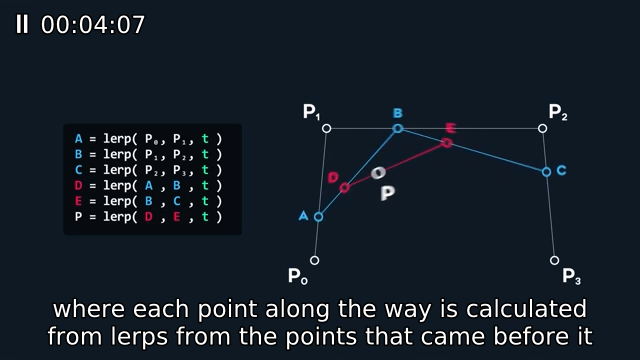
\includegraphics[width=5.5cm]{2021-2-C3/bezier_4:07.png}
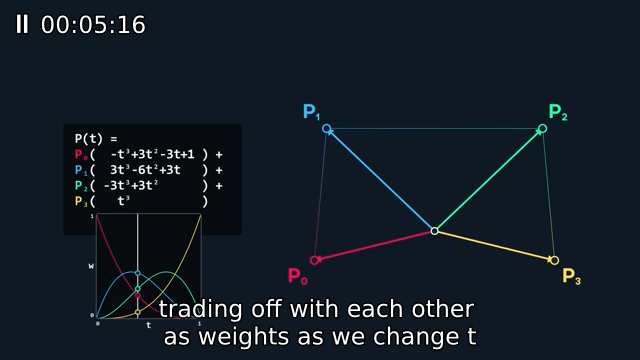
\includegraphics[width=5.5cm]{2021-2-C3/bezier_5:16.png}

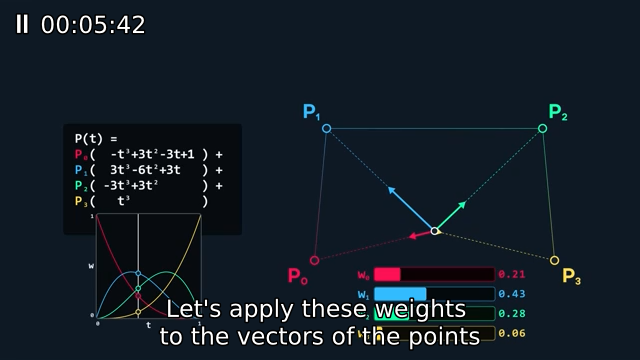
\includegraphics[width=5.5cm]{2021-2-C3/bezier_5:42.png}


\newpage

%  _____                         _     ____  
% | ____|_  _____ _ __ ___ ___  / |   |___ \ 
% |  _| \ \/ / _ \ '__/ __/ __| | |     __) |
% | |___ >  <  __/ | | (__\__ \ | |_   / __/ 
% |_____/_/\_\___|_|  \___|___/ |_( ) |_____|
%                                 |/         

{\bf Exercício 1}

Neste exercício vamos usar

$P_0=(1,1)$, $P_1=(1,2)$, $P_2=(3,2)$, $P_2=(3,5)$.

\ssk

Marque estes 4 pontos no $\R^2$ e escreva do lado de cada um dos
pontos o nome dele. Neste exercício vamos chamar o gráfico com esses 4
pontos e os nomes dele de ``diagrama básico'', e você vai precisar de
várias cópias do diagrama básico, uma pra cada item.

\msk

a) Seja $t=\frac12=0.5$. Encontre os pontos $A,B,C,D,E,P$ da
construção do frame 4:07 usando este valor de $t$ e marque esses
pontos na sua primeira cópia do diagrama básico. Escreva do lado de
cada ponto o nome dele.

b) Idem, mas na segunda cópia do diagrama básico e com $t=\frac14$.

c) Idem, mas na segunda cópia do diagrama básico e com $t=\frac34$.

\newpage

% «exercicio-2»  (to ".exercicio-2")
% (c3m212bezierp 6 "exercicio-2")
% (c3m212beziera   "exercicio-2")

{\bf Exercício 1 (cont.)}

d) Idem, mas em outra cópia, e usando $t=\frac18$. Agora só escreva o
nome do ponto $P$

e) Idem, mas usando $t=\frac38$.

f) Idem, mas usando $t=\frac58$.

g) Idem, mas usando $t=\frac78$.

\bsk

{\bf Exercício 2}

Agora veja se você consegue refazer todos os exercícios anteriores num
gráfico só sem desenhar os pontos auxiliares. Mais precisamente:
comece com $t=\frac12$, descubra no olho onde estão os pontos
$A,B,C,D,E,P$ para este valor de $t$ sem desenhá-los, e desenhe só o
ponto $P$, escrevendo ``$P_{\frac12}$'' do lado dele. Depois faça a
mesma coisa para $P_{\frac14}$ e $P_{\frac34}$, e depois para
$P_{\frac18}$, $P_{\frac38}$, $P_{\frac58}$, $P_{\frac78}$. Dica: você
pôr um dedo em cada um dos pontos $A, B, C, D, E$ se ajudar.



\newpage

%  _____                   _      _         _____ 
% | ____|_  _____ _ __ ___(_) ___(_) ___   |___ / 
% |  _| \ \/ / _ \ '__/ __| |/ __| |/ _ \    |_ \ 
% | |___ >  <  __/ | | (__| | (__| | (_) |  ___) |
% |_____/_/\_\___|_|  \___|_|\___|_|\___/  |____/ 
%                                                 
% «exercicio-3»  (to ".exercicio-3")
% (c3m212bezierp 7 "exercicio-3")
% (c3m212beziera   "exercicio-3")

{\bf Exercício 3.}

No PDF sobre vetores tangentes você fez três exercícios de desenhar
trajetórias curvas e os vetores tangentes delas em certos pontos. Eram
os exercícios 2, 3 e 4 daqui:

\ssk

{\footnotesize

% (c3m212vtp 6 "exercicio-2")
% (c3m212vta   "exercicio-2")
\url{http://angg.twu.net/LATEX/2021-2-C3-vetor-tangente.pdf}

}

\msk

Agora que o seu olhômetro está bem melhor nós vamos ver um modo de
desenhar aproximações pra esses trajetórias usando quase só desenhos e
fazendo pouquíssimas contas.


\newpage

% «exercicio-3-cont»  (to ".exercicio-3-cont")
% (c3m212bezierp 8 "exercicio-3-cont")
% (c3m212beziera   "exercicio-3-cont")

{\bf Exercício 3 (cont.)}

\ssk

\def\CA{\ColorRed}
\def\CB{\ColorOrange}
\def\CC{\ColorGreen}
\def\CD{\ColorViolet}

No exercício 2 do PDF de vetores tangentes nós tínhamos
$P(t) = (\cos t, \sen t)$; no exercício 3 tínhamos
$P(t) = (\cos t, \sen 2 t)$, e no exercício 4 tínhamos
$P(t) = (\cos 2t, \sen t)$. Vamos mudar os nomes para:
%
$$\begin{array}{ll}
  P(t) = (\CA{\cos t}, \CB{\sen t}),  & P'(t) = \VEC{\CC{-\sen t}, \CD{\cos t}} \\
  Q(t) = (\CA{\cos t}, \CB{\sen 2t}), & Q'(t) = \VEC{\CC{-\sen t}, \CD{2\cos 2t}} \\
  R(t) = (\CA{\cos 2t}, \CB{\sen t}), & R'(t) = \VEC{\CC{-2\sen 2t}, \CD{\cos t}} \\
  \end{array}
$$

Se usarmos quatro cores diferentes conseguimos representar pra cada
trajetória as componentes $x$ e $y$ dela e as componentes $x$ e $y$ da
derivada dela num gráfico só...

\newpage

% «exercicio-3-figs»  (to ".exercicio-3-figs")
% (c3m212bezierp 9 "exercicio-3-figs")
% (c3m212beziera   "exercicio-3-figs")

% (c2m211prp 5 "parabola-complicada")
% (c2m211pra   "parabola-complicada")
%L
%L sin, cos, pi = math.sin, math.cos,math.pi
%L -- ct = function (t) return cos(t) end
%L -- st = function (t) return sin(t) end
%L -- c2t = function (t) return cos(2*t) end
%L -- s2t = function (t) return sin(2*t) end
%L
%L -- pwi = Piecewisify.new(f_funcao_complicada, seq(0, 4, 0.25), 5, 6, 7)
%L -- pct  = Piecewisify.new(ct, seq(0, 2*pi, pi/16))
%L -- pst  = Piecewisify.new(st, seq(0, 2*pi, pi/16))
%L -- pc2t = Piecewisify.new(c2t, seq(0, 2*pi, pi/16))
%L -- ps2t = Piecewisify.new(s2t, seq(0, 2*pi, pi/16))
%L -- pmct  = Piecewisify.new(ct, seq(0, 2*pi, pi/16))
%L -- pmst  = Piecewisify.new(st, seq(0, 2*pi, pi/16))
%L -- pmc2t = Piecewisify.new(c2t, seq(0, 2*pi, pi/16))
%L -- pms2t = Piecewisify.new(s2t, seq(0, 2*pi, pi/16))
%L
%L PW = function (s) return
%L   Piecewisify.new(L("t -> "..s), seq(0, 2*pi, pi/32)):pw(0, 2*pi)
%L end
\pu

\def\trajcomponents#1{%
  \vcenter{\hbox{%
    \beginpicture(0,-2)(7,2)
    \pictgrid%
    #1%
    \pictaxes%
    \end{picture}%
  }}}

\unitlength=12pt

%$$\begin{array}{ll}
%  P(t) = (\CA{\cos t}, \CB{\sen t}),  & P'(t) = \VEC{\CC{-\sen t}, \CD{\cos t}} \\
%  Q(t) = (\CA{\cos t}, \CB{\sen 2t}), & Q'(t) = \VEC{\CC{-\sen t}, \CD{2\cos 2t}} \\
%  R(t) = (\CA{\cos 2t}, \CB{\sen t}), & R'(t) = \VEC{\CC{-2\sen 2t}, \CD{\cos t}} \\
%  \end{array}
%$$

$$\begin{array}{l}
    P(t) = (     \CA{ \cos t}, \CB{\sen t}) \\
    P'(t) = \VEC{\CC{-\sen t}, \CD{\cos t}} \\
  \end{array}
  \quad
  \trajcomponents{%
    \CA{\expr{PW" cos(t)"}}%
    \CB{\expr{PW" sin(t)"}}%
    \CC{\expr{PW"-sin(t)"}}%
    \CD{\expr{PW" cos(t+0.05)"}}%
  }
$$
$$\begin{array}{l}
    Q(t) = (     \CA{ \cos t}, \CB{ \sen 2t}) \\
    Q'(t) = \VEC{\CC{-\sen t}, \CD{2\cos 2t}} \\
  \end{array}
  \quad
  \trajcomponents{%
    \CA{\expr{PW"   cos(  t)"}}%
    \CB{\expr{PW"   sin(2*t)"}}%
    \CC{\expr{PW"-  sin(  t)"}}%
    \CD{\expr{PW" 2*cos(2*t)"}}%
  }
$$
$$\begin{array}{l}
    R(t) = (     \CA{ \cos 2t}, \CB{ \sen t}) \\
    R'(t) = \VEC{\CC{-2\sen 2t}, \CD{\cos t}} \\
  \end{array}
  \quad
  \trajcomponents{%
    \CA{\expr{PW"   cos(2*t)"}}%
    \CB{\expr{PW"   sin(  t)"}}%
    \CC{\expr{PW"-2*sin(2*t)"}}%
    \CD{\expr{PW"   cos(  t)"}}%
  }
$$

\newpage

% «exercicio-3-cont»  (to ".exercicio-3-cont")
% (c3m212bezierp 10 "exercicio-3-cont")
% (c3m212beziera    "exercicio-3-cont")

{\bf Exercício 3 (cont.)}

\def\hp{\frac{π}{2}} % halfpi


\scalebox{0.7}{\def\colwidth{8cm}\firstcol{

Copie cada uma dos três gráficos da página anterior -- cada um deles
tem quatro funções -- para uma folha de papel separada, mas com uma
modificação...

\ssk

Ao invés de desenhar as funções sobre um quadriculado em que as linhas
horizontais estão em $y=0$, $y=1$, $y=2$, $y=-1$ e $y=-2$ e as linhas
verticais estão em $x=0$, $x=1$, $x=2$, $\ldots$, desenhe um
``retangulado'' no qual as linhas verticais estão em $x=0$, $x=\hp$,
$x=2\hp$, $x=3\hp$, etc -- e depois use esses seus gráficos pra
refazer os exercícios 2, 3 e 4 do PDF de vetores tangentes ``no
olho'': agora ao invés de calcular cada seno e cada cossendo dos
exercícios 2, 3 e 4 por fórmulas e tabelas você vai descobrir os
valores deles pelos gráficos.

\ssk

}\anothercol{

Ah, repare que as coisas vermelhas no slide anterior representam a
\CA{posição horizontal} da trajetório, as em laranja representam a
\CB{posição vertical}, as em verde representam \CC{velocidade na
  horizontal} e as em roxo \CD{velocidade na vertical}. Quando
representarmos a vetor velocidade a velocidade na horizontal vai ser
representada como um deslocamento na horizontal e a velocidade na
vertical vai ser representada como um deslocamento na vertical... nós
vamos ver o porquê disto em breve.

}}


\GenericWarning{Success:}{Success!!!}  % Used by `M-x cv'

\end{document}

%  ____  _             _         
% |  _ \(_)_   ___   _(_)_______ 
% | | | | \ \ / / | | | |_  / _ \
% | |_| | |\ V /| |_| | |/ /  __/
% |____// | \_/  \__,_|_/___\___|
%     |__/                       
%
% «djvuize»  (to ".djvuize")
% (find-LATEXgrep "grep --color -nH --null -e djvuize 2020-1*.tex")

 (eepitch-shell)
 (eepitch-kill)
 (eepitch-shell)
# (find-fline "~/2021.2-C3/")
# (find-fline "~/LATEX/2021-2-C3/")
# (find-fline "~/bin/djvuize")

cd /tmp/
for i in *.jpg; do echo f $(basename $i .jpg); done

f () { rm -v $1.pdf;  textcleaner -f 50 -o  5 $1.jpg $1.png; djvuize $1.pdf; xpdf $1.pdf }
f () { rm -v $1.pdf;  textcleaner -f 50 -o 10 $1.jpg $1.png; djvuize $1.pdf; xpdf $1.pdf }
f () { rm -v $1.pdf;  textcleaner -f 50 -o 20 $1.jpg $1.png; djvuize $1.pdf; xpdf $1.pdf }

f () { rm -fv $1.png $1.pdf; djvuize $1.pdf }
f () { rm -fv $1.png $1.pdf; djvuize WHITEBOARDOPTS="-m 1.0 -f 15" $1.pdf; xpdf $1.pdf }
f () { rm -fv $1.png $1.pdf; djvuize WHITEBOARDOPTS="-m 1.0 -f 30" $1.pdf; xpdf $1.pdf }
f () { rm -fv $1.png $1.pdf; djvuize WHITEBOARDOPTS="-m 1.0 -f 45" $1.pdf; xpdf $1.pdf }
f () { rm -fv $1.png $1.pdf; djvuize WHITEBOARDOPTS="-m 0.5" $1.pdf; xpdf $1.pdf }
f () { rm -fv $1.png $1.pdf; djvuize WHITEBOARDOPTS="-m 0.25" $1.pdf; xpdf $1.pdf }
f () { cp -fv $1.png $1.pdf       ~/2021.2-C3/
       cp -fv        $1.pdf ~/LATEX/2021-2-C3/
       cat <<%%%
% (find-latexscan-links "C3" "$1")
%%%
}

f 20201213_area_em_funcao_de_theta
f 20201213_area_em_funcao_de_x
f 20201213_area_fatias_pizza



%  __  __       _        
% |  \/  | __ _| | _____ 
% | |\/| |/ _` | |/ / _ \
% | |  | | (_| |   <  __/
% |_|  |_|\__,_|_|\_\___|
%                        
% <make>

 (eepitch-shell)
 (eepitch-kill)
 (eepitch-shell)
# (find-LATEXfile "2019planar-has-1.mk")
make -f 2019.mk STEM=2021-2-C3-bezier veryclean
make -f 2019.mk STEM=2021-2-C3-bezier pdf

% Local Variables:
% coding: utf-8-unix
% ee-tla: "c3b"
% ee-tla: "c3m212bezier"
% End:
